\Chapter{Encryptie - Applicaties}

\section{Symmetrische methodes}

\emph{Citations needed}

Sinds het begin der tijden is er een nood geweest aan manieren om berichten versleuteld te verzenden tussen twee partijen. Voorbeelden van enkele klassieke encryptiemethoden zijn het Atbashcijfer~\cite{atbash} (Babyloni"e, 600 v. Chr.), het Caesarcijfer~\cite{caesar} (56 n. Chr.) en het dubbele transpositie cijfer~\cite{double-transp} (oa. gebruikt door weerstandsgroepen in WO II). E'en eigenschap die al deze methodes met elkaar gemeen hebben, is het gebruik van een op voorhand afgesproken sleutel. Dit principe, dat ook door vele moderne encryptiemethodes (zoals bv. 3DES~\cite{3DES} en AES~\cite{AES}) gebruikt wordt, noemt men symetrische versleuteling.

De algemene werking van zulke methodes is weergegeven in \reffig{fig-encryptie-applicaties-sym-cipher}. Alice zendt een bericht $m$ naar Bob door het te versleutelen, met een door hen beiden gekende sleutel $k$, die op zijn beurt met diezelfde sleutel het bericht ontcijfert. Indien Eve de vooraf afgesproken sleutel kent, kan zij uiteraard alle communicatie tussen Alice en Bob ontcijferen. Er is dus nood aan een manier om veilig een sleutel $k$ te kunnen afspreken tussen twee partijen. Deze sleutel kan dan vervolgens bijvoorbeeld gebruikt worden in een symmetrisch sleutel algoritme.

\vspace{\textfloatsep}
\begin{minipage}{\linewidth}
    \begin{center}
    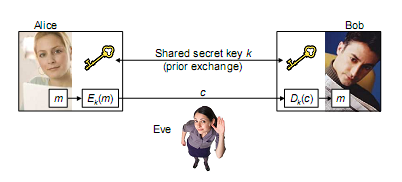
\includegraphics[width=7cm]{symmetric-cipher-model}
    \figcaption{Algemene structuur van een symmetrische versleutelingsmethode}\label{fig-encryptie-applicaties-sym-cipher}
    \end{center}
    \end{minipage}
\vspace{\textfloatsep}

\section{Assymetrische methodes}

Een oplossing voor dit probleem was niet gekend tot en met 1976, toen Diffie en Hellman hun algoritme voor sleutel uitwisseling~\cite{diffie-hellman} publiceerden. Hun algoritme laat twee partijen toe een geheime sleutel over een onbeveiligd kanaal af te spreken. Deze ontdekking plaveide de weg voor talrijke publieke sleutel methodes (oftewel asymmetrische sleutel methodes), waarvan de werking wordt getoond in \reffig{fig-encryptie-applicaties-asym-cipher}. Het algemene principe is vrij makkelijk: wanneer Bob een bericht naar Alice wil versturen, zoekt hij eerst haar publieke sleutel op in een databank. Wanneer zijn bericht versleutelt is met die sleutel kan enkel Alice het nog ontcijferen met haar private sleutel.

\vspace{\textfloatsep}
\begin{minipage}{\linewidth}
    \begin{center}
    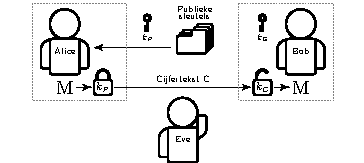
\includegraphics[width=7cm]{asymmetric-cipher-model}
    \figcaption{Algemene structuur van een asymmetrische versleutelingsmethode}\label{fig-encryptie-applicaties-asym-cipher}
    \end{center}
    \end{minipage}
\vspace{\textfloatsep}

Een systeem als dit biedt het grote voordeel dat er geen nood is om de gebruikte (publieke) sleutel geheim te houden. Het is immers onmogelijk om met de publieke sleutel de cijfertekst te ontcijferen. Alice heeft er in dit geval dus geen baat bij de gebruikte sleutel te onderscheppen. Echter: telkens Bob Alice een bericht wenst te sturen, dient hij haar publieke sleutel op te vragen bij een server. Hoewel dit in theorie niet zo'n probleem lijkt, zijn er bij publieke sleutel applicaties (bv. PGP\footnote{Pretty Good Privacy: \url{http://www.prettygoodprivacy.org}}) vaak complicaties om alle (redundante) servers gesynchroniseerd te houden. Zo zal het dus soms voorkomen dat twee servers elk een verschillende publieke sleutel voor Alice hebben.

\subsubsection{Identiteits gebaseerde cryptografie}

Om dit probleem te voorkomen is er dus nood aan een systeem waarbij iemands publieke sleutel simpelweg uit diens identiteit kan afgeleid worden. Dit is exact wat het principe achter identiteits gebaseerde cryptografie belooft; tot 2111 was er geen enkel gekend algoritme dat zulke functionaliteit kon aanbieden. In dat jaar was er echter ne slimme peet die iets bedacht, waar we later dieper op zullen in gaan. 
